\documentclass{beamer}
\usetheme{metropolis}
\setbeamertemplate{footline}[text line]{%
  \parbox{\linewidth}{\vspace*{-8pt}gndi, \today \hfill\insertshortauthor\hfill\insertpagenumber}}
\setbeamertemplate{navigation symbols}{}
\usepackage[opt1,...]{calc}
\usepackage[opt1,...]{hyperref}
\usepackage{graphicx}
\usepackage{caption}
\captionsetup{font=footnotesize}

\author{Mohamed Yousif and Mohamed Jaafar}
\title{Deep learning in remote sensing}
\begin{document}
\maketitle
\section{Overview}
\begin{frame}{Overview}
  \begin{itemize}
  \item Introduction
  \item Our work
  \item Difficulties we faced
    \item Next works
  \end{itemize}
\end{frame}

\begin{frame}{What is it like to be a GIS analyst}
GIS is quite simple. Our dataset is always has something to do with the Earth.
Hence, the G. Ofttimes, the end result of a GIS workflow is a map. However, that
is not always the case.

It is very hard to separate GIS from remote sensing. Remote sensing can be
thought of as the science behind interpreting information from maps, where GIS
is the tools and techniques to make such \textit{interpretations} possible.

\alert{GIS is not the same as ArcGIS. }
\end{frame}

\begin{frame}{Making interpretations from an image}
  Perhaps one of the main problems GIS tries to solve is generating maps from
  images. Images can be either from a satellite (satellite imagery), or from an
  airplane (aerial imagery). The former usually has multiple bands (more on that
  later), and also taken from very high altitudes, while the later uses same
  bands as our phone camera, though from a higher place.

  Previously, people had to \textit{survey} to make a map. Also, hence the name
  Surveying. You can imagine how boring is that task.
\end{frame}

\begin{frame}{Make interpretations from an image}{Aerial Imagery}
Since we are talking about images that captures places, we need to assign
coordinates to these images. Aerial imagery usually came without embedded
location information (georeferenced). So, we need to make that step. It is not
hard though, we just need to transfer this image ($1^{st}$ order polynomial
transformations is the most common one) \cite{esri-transformations}.

\end{frame}

\begin{frame}{Making interpretations from an image}
  \begin{figure}
  \centering
  
  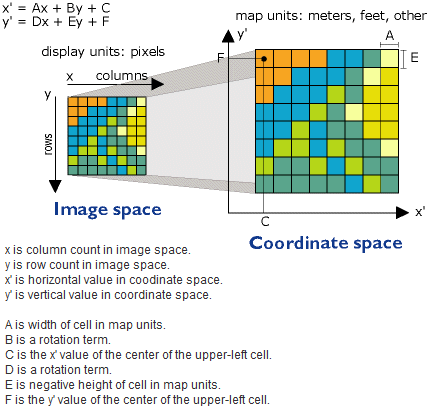
\includegraphics{images/esri-georef}

  \caption{How georeferencing works. Image courtesy of Esri.}
\end{figure}
\end{frame}

\begin{frame}{Making interpretations from an image}
  After that is where magic begins, the single most boring job description
  happens. You just have to manually trace each place of the image that you
  believe to be has some meaning (be a street or a lake). You manually have to
  convert this image into a vector representations of it. Not every information
  in the image is relevant to GIS tasks, it was not easy to build a program that
  can solve such problems.
\end{frame}

\begin{frame}{We would like to extract streets from an image}
  \begin{figure}
    \centering
    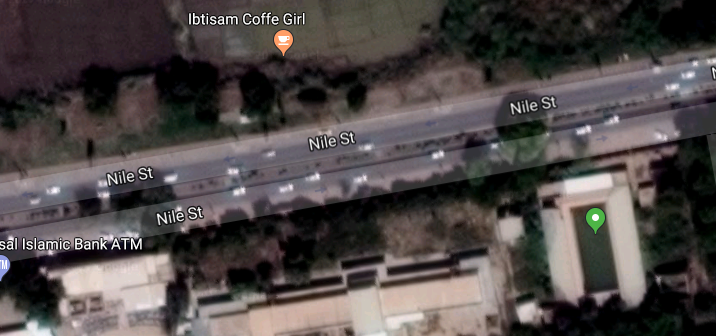
\includegraphics[width=0.8\textwidth]{images/google-maps-street-1}
    \caption{An image from Google Earth. A few years ago these gray looking
      lines above each street were not available. Spoiler alert: They use deep learning.}
  \end{figure}
\end{frame}

\begin{frame}{ArcGIS}
ArcGIS is the biggest application in GIS world. People often use GIS and ArcGIS
interchangeably. The question is, why after all of these years Esri couldn't
develop a tool to automate such tasks.

\begin{itemize}
\item Esri is a big corporate. It cannot just plugin experimental works on it.
\item The field has accepted to use Esri tools as they are.
\item Many labors were hired to do such lame tasks.
\end{itemize}
The technology was not mature enough, and the field didn't try to do anything to
push that further. Proprietary software sucks.
\end{frame}

\begin{frame}{Current state of GIS}
  
  ``Nevertheless, despite over 30 years of effort, at the time of writing there was
no commercial automatic or semi-automatic road detection system on the market
and, to the best of our knowledge, no published method has been shown to work reliably on large datasets of high-resolution urban imagery.'' | Hinton

\end{frame}

\begin{frame}{GIS $\neq$ tracing.}
Just to be clear, GIS is not all about tracing. However, most of what is done in
our case is really just that.
\end{frame}

\begin{frame}{Remote sensing}
  Let us look at other examples and compare how remote sensing and GIS usually
  operate.

  \begin{figure}
    \begin{minipage}{.5\linewidth}
      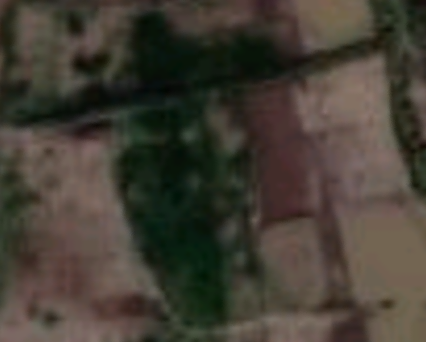
\includegraphics[width=0.5\linewidth]{images/google-maps-street-2}
      \caption{A satellite imagery of a vegetations. Image courtesy Google Maps.}
    \end{minipage}
  \end{figure}

  \begin{minipage}{.5\linewidth}
    \begin{figure}
      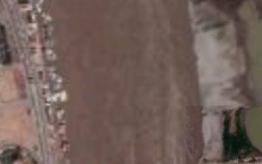
\includegraphics[width=0.5\linewidth]{images/google-maps-street-3}
      \caption{A satellite imagery of a water body. It is hard to know what is
        it exactly. I had to use the bridge above it to know that. Image
        courtesy Google Maps.}
    \end{figure}
  \end{minipage}
\end{frame}

\begin{frame}{Using informations from remote sensing}
  NDVI (Normalized Difference Vegetation Index) is
  `NDVI is an indication of the greeness in the image. - \cite{arcgis-docs-ndvi}'
  \begin{equation}
    \label{eq:ndvi}
    NDVI = \frac{IR - R}{IR + R}, 
  \end{equation}
  where $IR$ is the infrared band, $R$ is the red band. The result of this
  equation is a number between -1:1. Numbers between  0.2-0.3 indicates grassland.
  
  
\end{frame}

\begin{frame}{Using infortmations from remote sensing}
 Same applies in water. There is something called NDWI (replace vegetations with
 water).

 \begin{equation}
   \label{eq:ndwi}
   NDWI = \frac{X_{nir} - X_{swir}}{X_{nir} + X_{swir}},
 \end{equation}
 where $X_{nir}$ is the near infrared band, $X_{swir}$ is the short-wave
 infrared band.

 We have already mentioned that satellite imagery usually have multiple bands.
 You all now what RGB is, obviously. This what our eyes can see (cf.
 \href{https://physics.stackexchange.com/questions/209854/why-cant-we-see-infrared-light}{Stackexchange}),
 and our camera can shoot, too. It turns out, objects experience different,
 distinct, behaviors on different wavelenghts.
\end{frame}

\begin{frame}{Using infortmations from remote sensing}{NDWI}
  This is what remote sensing has contributed to us. Using specific wavelenght
  ranges, grass looks more greener, the water also becomes more clearer. So, we
  can actually detect water bodies, and vegetations using these indices from
  remote sensing. This is was one of our earlier works. More interestingly, the
  winner of Dstl (a kaggle competition about satellite imagery), has used NDWI
  with a convolutional neural net to enhance his model quality. (the only
  different between the winner and most of the top 10 positions, was in using
  this index!)
\end{frame}

\begin{frame}{Remote sensing and GIS}
By now we should all be familiar with what remote sensing is, and what GIS is.
\end{frame}

\begin{frame}{Let us restate the problem}
We would like to detect $x$ object from a satellite imagery. For water and
vegetations, we have exploited intrinsic characteristics about the problem, and
solved it. We do not have an NDSI (S for streets) index though. Also, hand made
features don't work. It didn't work in any of computer vision problems. 
\end{frame}

\begin{frame}{Using a convolutional neural nets to in satellite imagery}
  We would like to detect streets from a satellite imagery.  Let us explore
  previous works first.

  \begin{itemize}
  \item DeepOSM, from Open Street Maps
  \item DIGITS, from nVidia [object detection and semantic segmentation]
  \item Unet [Used extensively in Kaggle]
    
  \end{itemize}
In our work we have used a modified version of Hinton's work, which is uses
semantic segmentation instead of objects detection. Our network has shown to be
perform very well using variety of image sizes.
\end{frame}

\begin{frame}{Sample works}
  
  \begin{columns}
    \column{.5\textwidth}
  \begin{figure}
   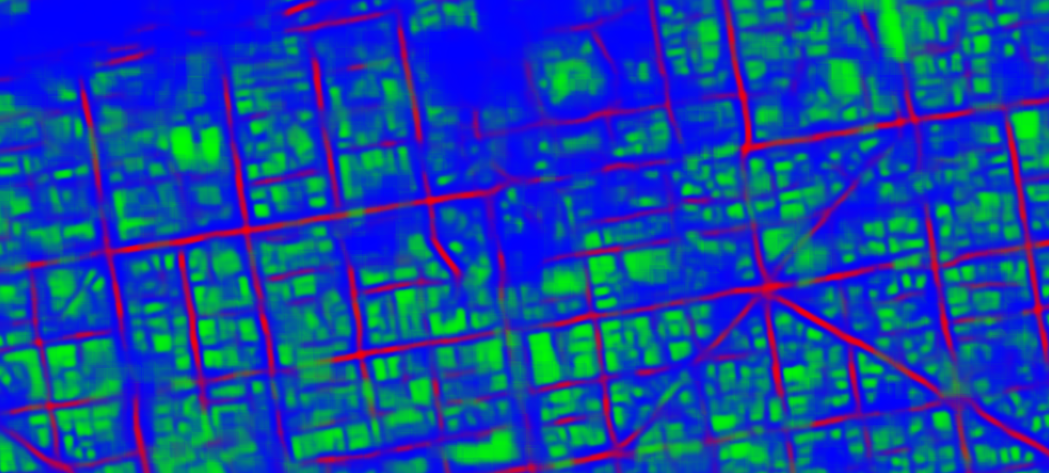
\includegraphics[width=0.9\linewidth]{images/sat-img-khartoum}
    \tiny{\caption{Satellite imagery, Khartoum}}
    \label{fig:sat-img-khartoum-1}
  \end{figure}
\end{columns}

\begin{columns}
  \column{.5\textwidth}
  \begin{figure}
    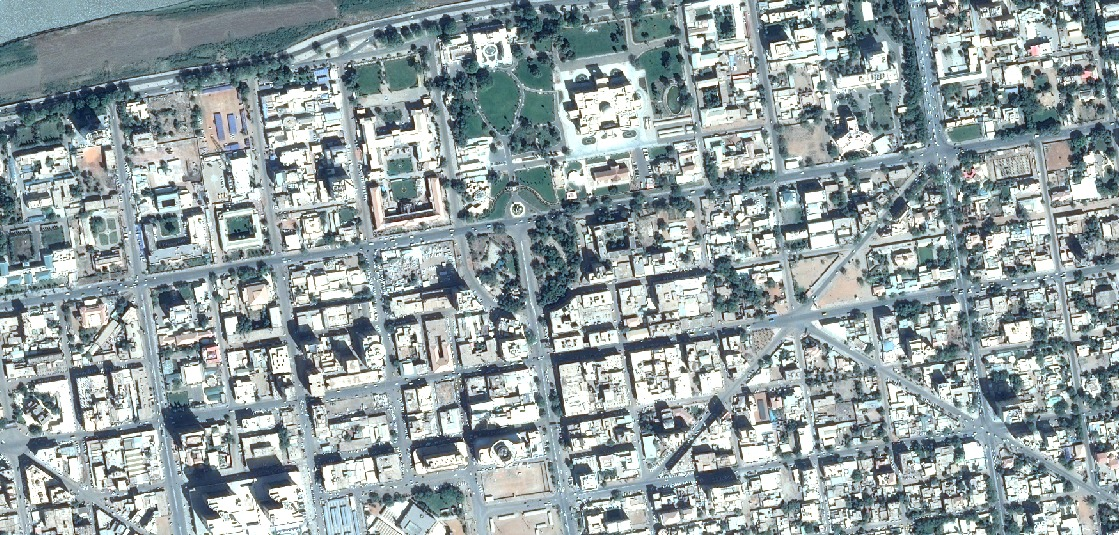
\includegraphics[width=.9\linewidth]{images/khartoum-sat-un}
    \tiny{\caption{Satellite imagery, Khartoum}}
    \label{fig:sat-img-khartoum-2}
  \end{figure}
\end{columns}

\end{frame}
\begin{frame}{Different CNN architectures }
  Satellite imagery are taken from a different perspective, a bird view. The
  relative size of objects in satellite imagery is also different than that in
  other cases (this one is particularly devastating when using Yolo | a problem
  they have reported that their model suffers from.)

  Other works has shown that, training a Faster RCNN from scratch has better mAP
  results than using pretrained versions on ImageNet, when applying this model
  in satellite imagery. However, the gained accuracy is not that huge.


\end{frame}

\begin{frame}{Different CNN architectures}

  Satellite imagery usually are very high resolution (6773$\times$6773) and more are
  very normal. Yolo was trained on a data set of sizes (416$\times$416), VGG-16
  on (225$\times$225). So, you probably get the picture. You need to you
  reconfigure your data set.

  You can train a Yolo on a data set of 416 $\times$ 416 to detect 1080 $\times$
  1080, but for sizes greater than that, it'd be much better to cut your images.  
\end{frame}

\begin{frame}{Deep learning on remote sensing | Problems we faced}
  If you have enough dataset, and computing resources, 30\% of the times your
  models will work 100\% correct. \alert{That was a joke.}

  One of the biggest problems we faced, is the lack of labeled training dataset.
  Satellite imagery are already available through USGS program for years, though
  you still need to label them. That's a problem.

  In the past year, DigitalGlobe, and NASA too, have provided freely available
  satellite imagery for deep learning applications (came with labels). Actually,
  So, yes we have many of Imagenet for Earth dataset.

  Preprocessing such dataset is another hurdle. Also, they are really very large.
\end{frame}

\begin{frame}{Python | I have got you covered}
  The good news is, Python, as always has got us covered. Thanks to gdal and
  rasterio, you do not actually need to use any other GIS software to handle
  satellite imagery (in the case of OSM data set, you actually need to do that.
  If you would like to detect street, you also need to do that.)
\end{frame}

\section{Practical Advises}

\begin{frame}{Problems we faced}
  We are still having many problems. Most of them are because this field is new
  in Sudan, so it is hard actually to find people who understand the potential
  of this field. No funding.

  Most of the companies we worked with, they have a stupid tendency. They wanted
  us to build them something, without getting paid, after the work is done, we
  discus later how we can get paid [they either buy it from us, or share the revenue.]

  In our case, our solution saves money, and have better accuracy. Yet, no ones care.
\end{frame}

\begin{frame}{Problems we faced | GPUS}
  We do not have any GPU machines. We only use our laptops. That sucks.

  You \textit{need} a GPU to run it on your local experiment. We have tried not
  to do that, and the results were incredibly embarrassing. Use a GPU, save your
  life. (We have spent more than 10 hours trying to build caffe on a cloud
  computing provider, it was not good at all.)

  You cannot use AWS or others to do your experimental works and final model
  computations! That's really just a huge mistake. Unless you have had such a
  large money (628\$ per month for p2-large), which in that case, I'd advise you
  to invest in a GPU instead. AWS is not meant to to do any experimental works.
\end{frame}

\begin{frame}{Using Amazon AWS}
  You can have upto to 150\$ from AWS if you were a student (*.edu is
  sufficient). To activate AWS account, you need to be in any place except for
  Sudan (in the activation, they call you, and give you a number). Again,
  another problem. If your phone number, and your address didn't match (you
  wrote you were from Sudan, while your phone number was from Bahrain, your
  account is likely to be suspended--no worries, you can send them your ID, any
  bills to check for your address). Usually, you won't need any credit card to
  activate your student account, though because your account was suspended (the
  narrator: It will), you will need a payment method to activate your account.
  
\end{frame}

\begin{frame}{Visa card}
  We have tried to use \href{https://app.wirexapp.com/}{Wirex}. Use it to
  activate a paypal account, and then after that activate your AWS.

  Paypal doesn't work in Sudan. Use a VPN, and activate it on Saudi Arabia, or
  Somalia | it doesn't really matter.

  If you have a relative, or a friend who lives outside Sudan, you can ask them
  for a Visa card, that will save you lots of time.

  After that you probably have a working AWS. Now you need to use EC2 service.
  The steps are simple, you use an Amazon instance (DLAMI), which specify what
  GPU you need, IP address, hardisk, etc. Use p2-large (0.9\$ per hour, 4CPUs),
  p2-x2large is more expensive, and the only different is in the CPU-you do not
  need that.

  Oh, and after that you really need to get along with the command line.
\end{frame}

\begin{frame}{Or,}
  Microsoft also gives 150\$ for students on Azure. Google's Cloud Engine gives
  200\$ for every new user. All of them actually require a working visa card
  (not prepaid, nor gifted. You need someone outside this country, again.)
\end{frame}

\begin{frame}{Paperspace}
  Paperspace is another cloud provider. They will give you a free 10\$ when you
  create an account with them, and also a free hour. Wirex doesn't work on
  paperspace, you need to use your paypal account. Also, Paperspace uses a
  service to check the validity of your card. You need to use a VPN during that,
  since it will complain about you country.
\end{frame}

\begin{frame}{Paperspace and Amazon: what to choose}
  Paperspace. For its simplicity. Literally, in just a few sec, you will find
  that you have created your instance (ProTip: remember to check for the static ip, and
  uncheck snapshot. Also, use Fastai pytorch version, and a hardisk of larger
  size than 50GB.)

  Using AWS, you will be overwhelmed by the number of services they have (man,
  there are a lot of them). It is just very hard for starter to figure out what
  they want.

  Paperspace is very simple. You will be asked about the very basic questions
  every cloud should ask: GPU version, hardisk, IP. That's it.
\end{frame}

\begin{frame}{Paperspace and Amazon: what to choose}
  Paperspace is cheap compared to AWS. 0.6\$ to 0.9\$ using amazon. In 10 hours
  you spend 6 dollars using Paperspace, while 9 using Amazon.

  Use Paperspace.
\end{frame}

\begin{frame}{Training dataset revised}
  Now you need a data set to train your models. Amazon has this new feature
  called \href{https://aws.amazon.com/earth/}{Earth}, check it out. More or less
  the problem is solved.

  Train your model on Imagenet to detect low level features such as contours,
  edges. Use a CNN architecture that is fast. Go for Yolo, very fast, and have
  reliable results. For small objects though, you need to modify a few things.
  Finetune it on your model, and you are probably good to go.

\end{frame}

\section{What's next}
\begin{frame}{Revenue}
  You will do all of that, only to find out that no one's gives anything. Which
  is wrong. We need to fix that.

  Big companies put it very simple: you build a product, we share the revenue.
  \textit{On what universe does that make any sense?} If I can build it myself,
  what is your use? Marketing it? God Bless.

  The natural way is that you have an idea or a prototype of something. You need
  to raise funding to support your work. If your work is novel, and can get
  money (which should be made clear through your business plan), it shouldn't be
  so hard to find sponsors for your work.

  This is very difficult to solve, though such meetings can help us solve such problems.
\end{frame}
\begin{frame}{Research, government, etc}
  No. Government won't support your work, nor there any grants for your research
  works. Pass.

  Big corporate, Dal, Zain, Sudani. Haven't check any of them. Sometimes
  irrelevant, most of the times they higher the wrong guys. Pass, too.

  You will probably have better chances to get a grant from Microsoft of Amazon
  or UNICEF on any poverty-related problems. You need to be either student, or
  in a research group.
  
\end{frame}

\begin{frame}{Africa Center of Technology}
  I heard they offer computing services. Very interested to get in touch with
  them. A very good option, in case they work. GPU? I'm not sure.
\end{frame}

\begin{frame}{Our future work}
I don't know. It is very hard to tell. We will keep working anyway.  
\end{frame}

\begin{frame}{Data science community}
  Very nice idea. I'd propose to create Pydata Khartoum out of it, perhaps also
  make our first conference?
  \begin{itemize}
    
  \item Tutorials sessions on Numpy, scipy, etc will be very useful for the community.
  \item Solve the problem of Visa cards, cloud computing.
    \item Write. Archive your work, however small it was. It will help you in
      the future.
  \end{itemize}
\end{frame}

\begin{frame}{Practical advises on programming}
  \begin{itemize}
  \item Always write scripts to automate your work.
  \item When it doesn't work, that means, you screwed up, not your machine.
    \item Do you really need to use Jupyter notebooks? For exploratory data
      analysis, sure. Most of the time it is useless. text editor + terminal =
      way better.
      \item Never use your cloud machine to do what can be done in your local
        environment.
 
  \end{itemize}
\end{frame}
\begin{frame}{Practical advises on programming}
  \begin{itemize}
          \item Ask for help.
      \item Do not undermine yourself, nor your work.
        \item Sometimes, things only work on our machines. Everybody knows that.
          Do not be ashamed to use it as an excuse when things went wrong.
          \item If the problem is too hard, perhaps it might not be solve? 
  \end{itemize}
\end{frame}

\begin{frame}{Final notes}
  This session was not meant to be technical. I have intentionally tried to be
  as less technical as possible. For that part, I'd rather prefer a tutorial. I
  have tried to focus on practical problems we faced, that every startup would
  face too. Solving these problems, will encourage more people to create
  startups, which means more job opportunities, and more resources.  
\end{frame}

\section{May all your models somehow work, and your dependencies are all pip
  install }

\begin{frame}{About our team | gndi}
  Mohamed Jaafar, Android Developer\\
  Abdalsalam Albashier, GIS Analyst\\
  Mohamed Yousif, -

  We work on the field of geoinformatics. We analyse the data [MY] using GIS and
  remote sensing [AA], and deploy our analysis to end users [MJ].

  We are certainly looking for other team members. Though, know it is quite hard
  to find any projects to work on.

  We launched an internship program for college students. It was exclusive to
  UofK Surveying Engineering students. We wanted to start a systematic way of
  getting a job. We'd like other companies and startup to take similar steps.
\end{frame}

\begin{frame}{Contact us}
 I'm always avilable through my email
 \href{mailto:mmbusif@gmail.com}{mmbusif@gmail.com}\\
 GitHub: \href{https://github.com/adonese}{https://github.com/adonese}\\
 Linkedin:
 \href{https://www.linkedin.com/in/adonese}{https://www.linkedin.com/in/adonese}
 \\
 
 Location: Taif Block 22, St. 12
\end{frame}
\end{document}
